\chapter{相關應用}

\section{電子鼻}
\subsection{人類嗅覺的限制}
即使在現代科技中,依然有許多行業需要依靠人體的嗅覺作為判斷依據。曾經有人做過
一個紅酒實驗 \cite{hodgson_2008} ,他觀察了許多種紅酒,發現同一種紅酒在兩次
紅酒競賽獲得的成績,其相關性不高。此外,人體的感官也可能因為感官疲勞而產生誤差。
因此,依靠人類的感官作為判斷依據的可靠度值得懷疑。
\subsection{原理}
電子鼻是一種用來模擬鼻子功能的電子儀器。利用多個感測器組合而成的一個整體,
而氣體在接觸到電子鼻時,內部的每個感測器會產生不同程度的電阻變化,因此透過
比對不同變化,即可產生電子指紋圖(electronic fingerprint)並辨識出
此為何種氣體,更甚者可計算出該氣體濃度。 \footnote{\url{https://scitechvista.nat.gov.tw/Article/C000003/detail?ID=e1893f7f-9eda-4ed7-ada0-dc226bfc1d57}}
\subsection{應用}
隨著科技演進,越來越多技術可以應用在電子鼻上。舉例來說,人工智慧可以運用
在電子鼻上, \footnote{\url{https://case.ntu.edu.tw/blog/?p=36043}}
\begin{figure}[H]
	\centering
	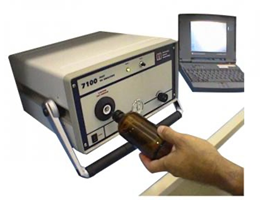
\includegraphics[width=0.5\textwidth]{../../pic/nose.png}
\end{figure}

\section{Alpla MOS}
Alpha MOS 由 6 個氣體感測器陣列所組成的 RQBOX 模組氣體監測系統,具有無線訊號傳輸裝置,
模組內的無線傳輸裝置可提供即時的遠端訊號傳輸,實際測試的結果顯示,其傳輸距離可達三百多公尺遠。
藉由連接有訊號接收器的電腦,可以提供遠端遙控即時空氣品質監測的功能。\footnote{\url{https://www.tiri.narl.org.tw/Files/Doc/Publication/InstTdy/145/01450060.pdf}}

\section{感知比較實驗}
進行人的嗅覺系統對於臭氣的感知比較實驗(三點比較式嗅袋法)- 人體嗅覺是否能察覺有害氣體。\footnote{\url{https://www.tiri.narl.org.tw/Files/Doc/Publication/InstTdy/145/01450060.pdf}}

\section{氣味感測器實例應用}
	\subsection{油管漏油事件}
	輸油管不論是遭受意外或人為蓄意破壞,漏油所影響的面積和環境污染程度最為嚴重。
	應用電子鼻分析結果。顯示整合現場快速判定未知樣品之電子鼻分析技術,協助取得代表性樣品,
	藉由 GC-MS 確認分析,同時達到緊急應變處置,降低災害至最低。\footnote{\url{https://www.tiri.narl.org.tw/Files/Doc/Publication/InstTdy/145/01450060.pdf}}
	\subsection{辦公大樓室內空氣異味事件}
	2002 年 11 月前往內疑有異味且地面有異物之辦公大樓,進行採樣檢測以了解可能原因。\footnote{\url{https://www.tiri.narl.org.tw/Files/Doc/Publication/InstTdy/145/01450060.pdf}}
	\subsection{羊乳摻牛乳事件}
	使用儀器分析羊乳中是否有牛乳摻假,多利用羊、牛乳中之脂肪酸或蛋白質(酪蛋白或乳清蛋白)組分之差異。
	使用電子鼻具有檢測時間短、檢測方法簡單、操作方法容易等優點。\footnote{\url{https://www.tiri.narl.org.tw/Files/Doc/Publication/InstTdy/145/01450060.pdf}}